\section{Werkzeuge der Bildverabreitung}
Die folgende Einleitung in die Thematik basiert auf der Lektüre des Buches
"Digitale Bildverarbeitung" von Burger, Burge \citep{burgeDigitBild}, das als 
Literatur für den Einstieg empfohlen wird. Eine zusammenfassende Wiedergabe für 
das Peojekt relevanter Themene ist im Folgenden nachzulesen.\\
Ein Bestandteil der Bildverarbeitung ist die Bildanalyse, bei der es darum geht,
sinnvolle Informationen aus Bildern zu extrahieren. Genauer ist der Bereich der
Computer Vision gefragt, die Sehvorgänge des Menschen in der dreidimensionalen Welt
zu mechanisieren.\\
Die Steuerung des Wagens soll durch Informationen aus den Kamerabildern
erfolgen: Durch Erkennen der Fahrbanhlinien soll die Lenkung innerhalb der Spur
geregelt werden.\\
Dieser Prozess lässt sich beschreiben mit:
\begin{enumerate}
  \item Digitalisierung mit Hilfe der Kamera
  \item Vorverarbeitung (Bildverbesserung bzw. Anpassung an den Zweck) durch
    Umwandlung in ein binäres Canny-Edges-Bild
  \item Segmentierung eine Vorauswahl des Bildauschnittes mit den relevante
    Informationen
  \item Merkmalsextraktion zur Linienerkennung durch die Hough-Transformation
  \item Parametrisierung als mathematische  Beschreibung der Fahrbahnlinien zur
    weiteren Informationsverarbeitung
\end{enumerate}

\subsection{Digitalisierung}
Der von der Kamera aufgenommen Bilder-Stream liegt in digitaler Form vor. Dabei lassen
sich benötigte Parameter eintellen(ergänzen Fabian?). Um ein optimales Bild zu
erhalten sind die Beleuchtungsumstände zu beachten, da hierdurch die
Differenzierung von Linien im Bild beeinflusst wird. Beachte timing? \\
In der Bildverabreitung ist der Nullpunkt der x- und y-Achse in der linken
oberen Ecke des Bildes definiert, was für ein eindeutiges Anwenden von Prozessen
und daraus generierten Informationen relevant ist.

\subsection{Vorverarbeitung- Canny-Kantenoperator}
Zur späteren Erkennung der Linien werden die dafür relevanten Informationen aus
dem Bild gefiltert: sogenannte Bildkannten. Bildkanten sind Übergangsstellen, wo
ein hoher Grauwertsprung von einem Pixel zum Nachbarpixeel erfolgt, wie z. B. bei 
einem weißen Farbahnstreifen zwei Kannten erkannt werden sollen.\\
Die Canny-Edges-Funktion aus der openCV Library ist ein bewährter Algorithmus zur Kantenerkennung, da drei Ziel
gleichzeitig erreicht werden drei Zile: ein zuverlässiges Detektieren
vorhandener Kanten, die Position der Kante präzise zu bestimmen, und Farbsprünge, 
die nicht als Kante interoretiert werden sollen, auszulassen.\\

\subsection{Segmentierung}
[BILD Kamera mit Fahrbahnlinien]
Der für die Erkennung der Fahrbahnlinien relevante Bereich liegt in einem
unteren Dreieck des Kamerabildes. Dieser Teil wird ausgewählt, bzw. davon ausserhalb
liegende Bereiche werden nicht bei der Erkennenung der Farbahnlinien
berücksichtigt.\\

\subsection{Merkmalsextraktion zur Linienerkennung}
Das Canny-Kantenbild wird mit Hilfe der Hough-Transformation aus der
openCV-Library in den Hough-Raum transformiert, wo dann die Erkennung der Linien
erfolgt.

\begin{minipage}{\columnwidth}
  \makeatletter
  \def\@captype{figure}
  \makeatother
  \centering
  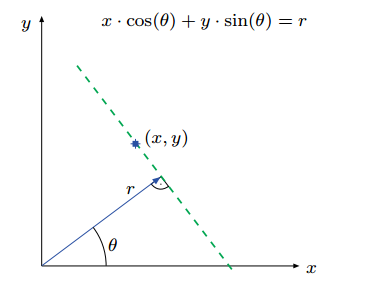
\includegraphics[width=0.8\linewidth]{images/gradeThetaR.png}
  \caption{gradeThetaR.png}
  \label{fig:gradeThetaR}
\end{minipage}

Dabei kommt zur Anwendung, dass eine Gerade mathematisch sowohl mit $y
= m \dot x + b$ als auch mit $r(\theta) = x \cdot cos(\theta) + y \cdot
sin(\theta)$ beschrieben werden kann. Dabei ist in der zweiten Beschreibung 
$\theta$ der  Winkel des Radius $r$ zum Urspung, an dessen Ende senkrecht die
beschriebene Grade verläuft. Zu Bedenken ist, dass wie schon erwähnt der
Koordinatenursprung des Bildes oben links definiert ist.\\
Das rechenaufwendige Verfahren der Hough-Transformation generiert für jeden
Kantenbildpunkt des Canny-Edges-Bildes Bildpunkte im Hough-Raum, dessen Achsen
ein $\theta$ / $r$ - Koordinatensystem bilden. Linien im kartesisches System
sind als Punkthäufungen im Hough-Raum erkennbar. Liegt eine Anzahl von
Punkten oberhalb eines zu definierenden Schwellwertes, wird eine Linie erkannt
und die Houh-Transformationsfunktion gibt ein Wertpaar $\theta$, $r$ zurück.
